% Figura 1 — visão geral da arquitetura da janela F7.
% Paleta e traço seguem o dossiê §5: tinta 1F2933, acento 0F766E, alerta B45309,
% fundo F5F7F8; sem gradiente, sem sombra, sem 3D.
\documentclass[11pt,tikz,border=6pt]{standalone}
% Fontes do bundle do TeX por NOME DE ARQUIVO: o `fontconfig` desta máquina não
% carrega a configuração padrão, então a busca por nome de família cairia em
% fallback silencioso. O .otf é resolvido pelo kpathsea e não usa fontconfig.
\usepackage{fontspec}
\setmainfont{LibertinusSerif}[Extension=.otf, UprightFont=*-Regular,
  BoldFont=*-Bold, ItalicFont=*-Italic, BoldItalicFont=*-BoldItalic, Ligatures=TeX]
\setmonofont{Inconsolatazi4-Regular}[Extension=.otf, BoldFont=Inconsolatazi4-Bold,
  Ligatures=TeX, Scale=0.92]
\usetikzlibrary{arrows.meta,fit,calc,shapes.geometric}

\definecolor{tinta}{HTML}{1F2933}
\definecolor{petroleo}{HTML}{0F766E}
\definecolor{ambar}{HTML}{B45309}
\definecolor{fundo}{HTML}{F5F7F8}

\begin{document}
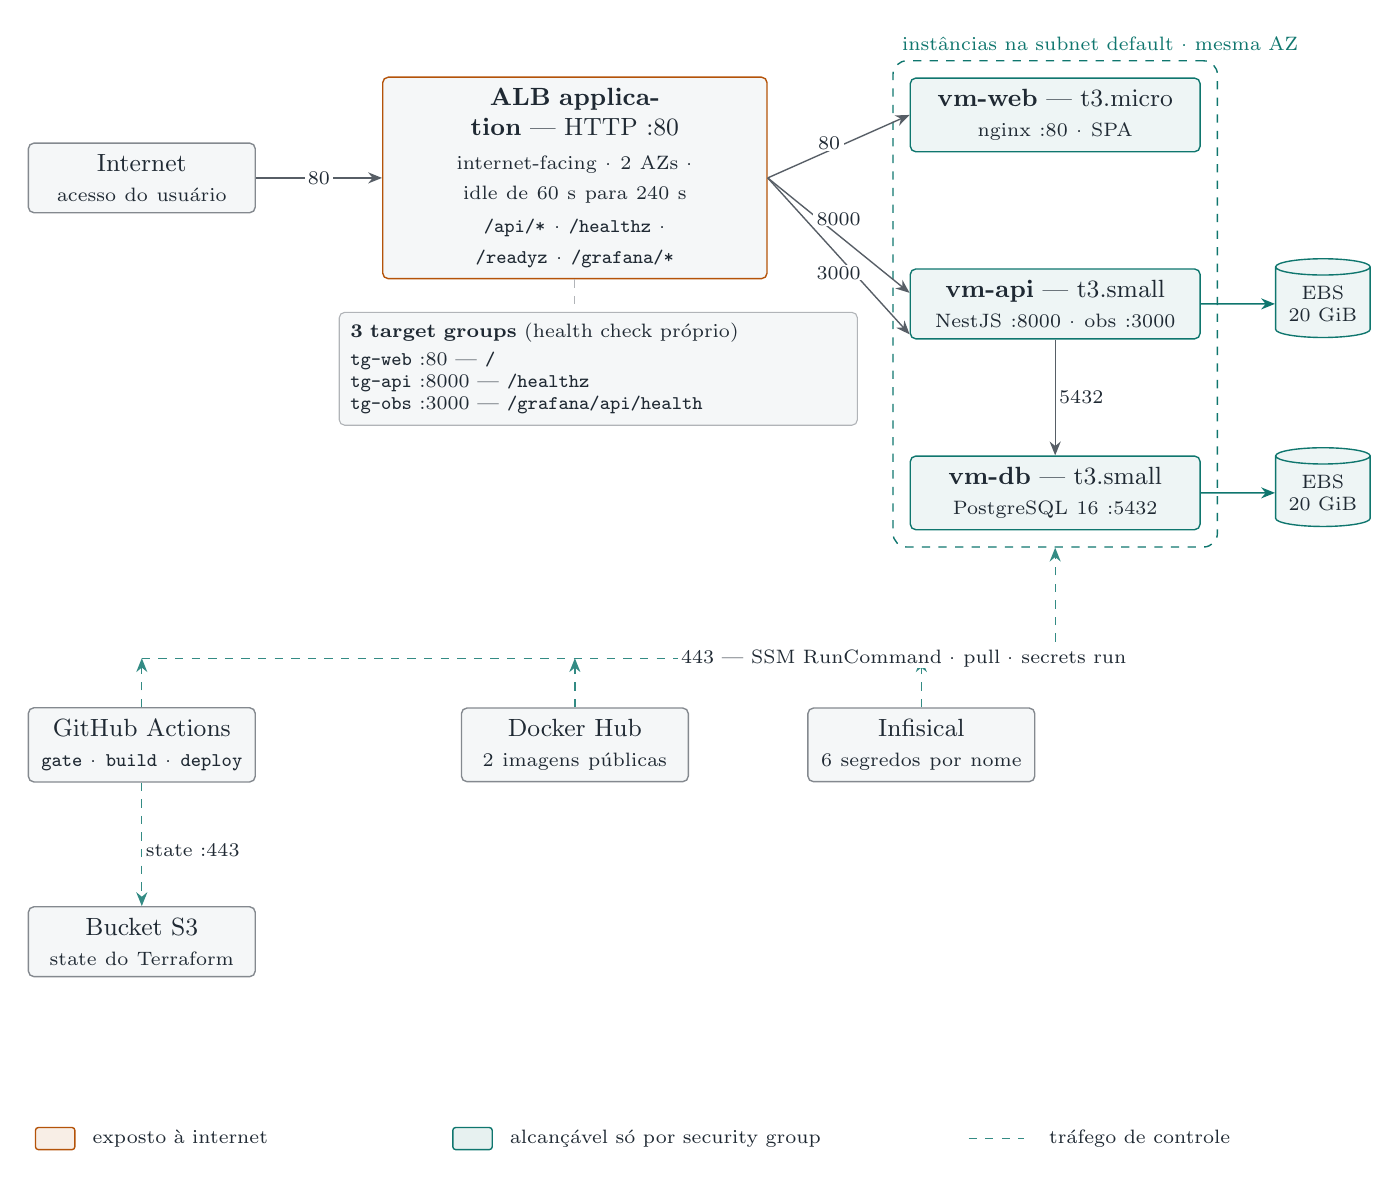
\begin{tikzpicture}[
    font=\small,
    >={Stealth[length=5pt,width=4pt]},
    pub/.style={draw=ambar, line width=0.5pt, fill=fundo, rounded corners=2pt,
      align=center, inner sep=4pt, text=tinta},
    priv/.style={draw=petroleo, line width=0.5pt, fill=petroleo!7, rounded corners=2pt,
      align=center, inner sep=4pt, text=tinta},
    ator/.style={draw=tinta!55, line width=0.5pt, fill=fundo, rounded corners=2pt,
      align=center, inner sep=4pt, text=tinta},
    nota/.style={draw=tinta!35, line width=0.4pt, fill=fundo, rounded corners=2pt,
      align=left, inner sep=4pt, text=tinta, font=\scriptsize},
    disco/.style={cylinder, shape border rotate=90, aspect=0.22, draw=petroleo,
      line width=0.5pt, fill=petroleo!7, align=center, inner sep=1pt,
      minimum height=1.0cm, minimum width=1.2cm, font=\scriptsize, text=tinta},
    seta/.style={->, line width=0.5pt, draw=tinta!75},
    ctrl/.style={->, dashed, line width=0.5pt, draw=petroleo!85},
    rot/.style={font=\scriptsize, text=tinta, fill=white, inner sep=1.2pt, inner ysep=0.5pt},
  ]

  % ---------- entrada pública ----------
  \node[ator, text width=2.6cm] (net) at (2.1,10.6)
    {Internet\\{\scriptsize acesso do usuário}};
  \node[pub, text width=4.6cm] (alb) at (7.6,10.6)
    {\textbf{ALB application} — HTTP :80\\[1pt]
     {\scriptsize internet-facing · 2 AZs · idle de 60 s para 240 s}\\[1pt]
     {\scriptsize \texttt{/api/*} · \texttt{/healthz} · \texttt{/readyz} · \texttt{/grafana/*}}};

  % ---------- os três target groups, com o health check de cada um ----------
  \node[nota, text width=6.3cm, anchor=north west] (tg) at (4.6,8.9)
    {\textbf{3 target groups} (health check próprio)\\[2pt]
     \texttt{tg-web} :80 — \texttt{/}\\
     \texttt{tg-api} :8000 — \texttt{/healthz}\\
     \texttt{tg-obs} :3000 — \texttt{/grafana/api/health}};
  \draw[draw=tinta!35, line width=0.4pt, dashed] (alb.south) -- (tg.north -| alb.south);

  % ---------- as três VMs, uma por papel ----------
  \node[priv, text width=3.4cm] (web) at (13.7,11.4)
    {\textbf{vm-web} — t3.micro\\{\scriptsize nginx :80 · SPA}};
  \node[priv, text width=3.4cm] (api) at (13.7,9.0)
    {\textbf{vm-api} — t3.small\\{\scriptsize NestJS :8000 · obs :3000}};
  \node[priv, text width=3.4cm] (db) at (13.7,6.6)
    {\textbf{vm-db} — t3.small\\{\scriptsize PostgreSQL 16 :5432}};

  \node[disco] (ebsapi) at (17.1,9.0) {EBS\\20 GiB};
  \node[disco] (ebsdb)  at (17.1,6.6) {EBS\\20 GiB};

  \node[draw=petroleo, dashed, line width=0.5pt, rounded corners=5pt,
        inner sep=6pt, fit=(web)(api)(db)] (grupo) {};
  \node[font=\scriptsize, text=petroleo, anchor=south west] at (grupo.north west)
    {instâncias na subnet default · mesma AZ};

  % ---------- cadeia de suprimento e de controle ----------
  \node[ator, text width=2.6cm] (gh) at (2.1,3.4)
    {GitHub Actions\\{\scriptsize \texttt{gate} · \texttt{build} · \texttt{deploy}}};
  \node[ator, text width=2.6cm] (s3) at (2.1,0.9)
    {Bucket S3\\{\scriptsize state do Terraform}};
  \node[ator, text width=2.6cm] (dh) at (7.6,3.4)
    {Docker Hub\\{\scriptsize 2 imagens públicas}};
  \node[ator, text width=2.6cm] (inf) at (12.0,3.4)
    {Infisical\\{\scriptsize 6 segredos por nome}};

  % ---------- arestas de tráfego ----------
  \draw[seta] (net.east) -- node[rot] {80} (alb.west);
  \draw[seta] (alb.east) -- node[rot,above left=-2pt] {80} (web.west);
  \draw[seta] (alb.east) -- node[rot,above=3pt] {8000} ([yshift=4pt]api.west);
  \draw[seta] (alb.east) -- node[rot,below=3pt] {3000} ([yshift=-11pt]api.west);
  \draw[seta] (api.south) -- node[rot,right] {5432} (db.north);
  \draw[seta, petroleo] (api.east) -- (ebsapi.west);
  \draw[seta, petroleo] (db.east) -- (ebsdb.west);

  % ---------- arestas de controle (443, de saída das VMs) ----------
  \draw[ctrl] (gh.north) -- (2.1,4.5);
  \draw[ctrl] (dh.north) -- (7.6,4.5);
  \draw[ctrl] (inf.north) -- (12.0,4.5);
  \draw[ctrl] (2.1,4.5) -- (13.7,4.5) -- (grupo.south);
  \node[rot, anchor=west] at (8.9,4.5) {443 — SSM RunCommand · pull · secrets run};

  \draw[ctrl] (gh.south) -- node[rot,right,pos=0.55] {state :443} (s3.north);

  % ---------- legenda ----------
  \node[draw=ambar, fill=ambar!10, minimum width=0.5cm, minimum height=0.28cm,
        line width=0.5pt, rounded corners=1pt] at (1.0,-1.6) {};
  \node[anchor=west, font=\scriptsize, text=tinta] at (1.35,-1.6) {exposto à internet};
  \node[draw=petroleo, fill=petroleo!10, minimum width=0.5cm, minimum height=0.28cm,
        line width=0.5pt, rounded corners=1pt] at (6.3,-1.6) {};
  \node[anchor=west, font=\scriptsize, text=tinta] at (6.65,-1.6)
    {alcançável só por security group};
  \draw[dashed, petroleo!85, line width=0.5pt] (12.6,-1.6) -- (13.3,-1.6);
  \node[anchor=west, font=\scriptsize, text=tinta] at (13.5,-1.6) {tráfego de controle};

\end{tikzpicture}
\end{document}
